\documentclass[conference]{IEEEtran}
\usepackage[hidelinks,hypertexnames=false]{hyperref}
\usepackage{graphicx}
\usepackage{cite}
\usepackage{float}
\usepackage{enumitem}
\usepackage{booktabs}
\usepackage{array}
\usepackage{url}
\usepackage{amsmath}
\usepackage{xcolor}
\usepackage{tikz}
\usetikzlibrary{arrows.meta,positioning}

\title{SimpleChef: Progress Report\\Human--Computer Interaction (CS4063)}
\author{%
\IEEEauthorblockN{[Group Name]}
\IEEEauthorblockA{[Institution / Course Section]\\
Email: [contact email]}}

\begin{document}
\maketitle

\begin{abstract}
This progress report summarizes development of SimpleChef, a mobile-first cooking assistant built with React Native (Expo), FastAPI, and PostgreSQL. We describe objectives aligned with our earlier proposal, implemented features as of March~22,~2026, known gaps relative to the proposed interface, ongoing design and engineering challenges, evidence placeholders for screenshots, remaining work, workflow and architecture figures, and an updated milestone timeline toward final delivery.
\end{abstract}

\section{Project Overview}
SimpleChef is a mobile-first cooking assistant designed to reduce friction across the entire cooking process---from discovering a recipe to meal planning and grocery shopping. The tagline \emph{Your calm kitchen companion} reflects the goal of a capable, calm tool that streamlines everyday cooking tasks.

As stated in our project proposal, many cooking apps fragment the experience: recipes in one place, calories in another, grocery lists on paper or in notes. Instructions often appear as long blocks of text, and timers frequently push users out of the recipe context. SimpleChef targets a single cohesive flow: recipe discovery, step-by-step cooking with integrated timers, meal planning with calorie awareness, and grocery support. The design applies HCI ideas including progressive disclosure, clarity over clutter, and smart defaults with full user control~\cite{preece2015,hartson2012ux}.

\subsection{Objectives (aligned with the proposal)}
\begin{itemize}[leftmargin=*]
  \item \textbf{Unify the workflow} across browsing, cooking mode, planning, and groceries with consistent navigation and data flow.
  \item \textbf{Optimize step-by-step cooking} so each step is scannable during active cooking, with integrated timers and (in the full design) mise en place tied to steps.
  \item \textbf{Timer management} via a timer dock that surfaces active timers without leaving the cooking context.
  \item \textbf{Grocery automation} from planned meals (deduplication, categories, editing, export) as a later integration milestone.
  \item \textbf{Lower recipe input friction} via manual entry plus AI-assisted text parsing with verification before save; image and video import remain planned.
  \item \textbf{Meal planning and calorie goals} by assigning meals to days and relating plans to profile goals; dietary filtering and richer statistics are extensions.
  \item \textbf{Iterate with users} through feedback sessions and refinement of flows and visuals~\cite{nielsen1994heuristic}.
\end{itemize}

\subsection{Tools and technology}
\begin{itemize}[leftmargin=*]
  \item \textbf{Frontend:} React Native (Expo) for cross-platform mobile development. Primary screens live under \texttt{frontend/app/} (e.g., tab routes for Home, Calendar, Add, Grocery, Profile; stack routes for recipe detail, cooking mode, manual entry).
  \item \textbf{Backend:} FastAPI (Python) with SQLAlchemy models and Alembic migrations; JWT auth for protected routes (\texttt{backend/app/api/}).
  \item \textbf{Data store:} PostgreSQL (via Docker Compose for local development).
  \item \textbf{Design:} Figma for wireframes and high-fidelity exploration~\cite{figma2026help}.
  \item \textbf{AI/ML:} Planned for parsing text, images, or video; the current server uses a structured placeholder parser in \texttt{backend/app/services/ai\_service.py} to exercise parse-then-edit UX end to end.
\end{itemize}


\section{Project Progress Overview}
As of March~22,~2026, the team has moved from specification into \textbf{working vertical slices}: an Expo client, FastAPI API, and PostgreSQL database support authenticated use of the main tabs and core flows described in the proposal.

\subsection{Completed milestones and components}
\begin{itemize}[leftmargin=*]
  \item \textbf{Proposal and design specification:} Scope, problem statement, five-tab UI (Home, Calendar, Add, Grocery, Profile), wireframe, and timeline documented.
  \item \textbf{Backend foundation:} Application entry (\texttt{main.py}, \texttt{run.py}), models for users, recipes (ingredients, steps), meal plans, grocery lists/items, and versioned migrations.
  \item \textbf{Authentication:} Signup and login on the client; JWT attached via an Axios interceptor (\texttt{frontend/services/api.ts}); protected creation of recipes and user-scoped grocery access patterns begun.
  \item \textbf{Recipe library (Home):} Scrollable list of recipe cards (\texttt{RecipeList}, \texttt{RecipeCard}) opening recipe detail by id.
  \item \textbf{Recipe detail:} Hero image when \texttt{image\_url} is set, summary stats, ingredients, and steps; \textbf{Begin Cooking} navigates to step-by-step mode (\texttt{app/recipe/[id].tsx}, \texttt{app/cooking/[id].tsx}).
  \item \textbf{Cooking mode:} One step at a time with previous/next, progress bar, optional per-step timer start when \texttt{timer\_seconds} is defined; \texttt{TimerDock} shows active timers sorted by least time remaining with play/pause and dismiss (see \texttt{TimerDock.tsx} and \texttt{useTimerStore.ts} under \texttt{frontend/}).
  \item \textbf{Add recipe:} Manual form with dynamic ingredient and step rows and optional timer fields per step (\texttt{app/add/manual.tsx}); paste flow opens a modal, calls \texttt{POST /recipes/parse}, and pre-fills the manual screen for verification (\texttt{app/(tabs)/add.tsx}). Image scan is a disabled \emph{Coming Soon} control.
  \item \textbf{Meal planner:} API range query and create plan; UI lists entries for a selected date and supports quick add of custom food name and calories (\texttt{app/(tabs)/calendar.tsx}). The \texttt{MealPlan} model supports \texttt{recipe\_id}; the current UI emphasizes quick-add over picking from the library.
  \item \textbf{Grocery list:} Per-user list, items grouped by category in a sectioned list, checkbox state persisted through the API, manual add modal (\texttt{app/(tabs)/grocery.tsx}, \texttt{endpoints/grocery.py}).
  \item \textbf{Profile:} Displays name, email, and calorie goal from \texttt{GET /users/me} (\texttt{app/(tabs)/profile.tsx}). Schema fields such as \texttt{dietary\_restrictions} exist for future editing and filtering.
\end{itemize}

\subsection{Gaps relative to the proposed UI}
\begin{itemize}[leftmargin=*]
  \item \textbf{Home:} Search and filter icons in the app bar are not wired to queries or client-side filters.
  \item \textbf{Cooking mode:} Per-step mise en place is not modeled (\texttt{Ingredient} is not linked to \texttt{Step}); the screen emphasizes instruction text and timers only.
  \item \textbf{Calendar:} Proposal called for a monthly grid with indicators and a bottom panel to add meals from the library; the current UI is a date-centric list with quick-add only.
  \item \textbf{Grocery:} No server or client pipeline yet to aggregate ingredients from planned recipes (deduplication, scaling, categories).
  \item \textbf{AI parsing:} Deterministic mock output, not a production LLM or vision pipeline---sufficient for flow testing only.
  \item \textbf{Profile:} No in-app editing of restrictions, goals, or social features despite partial schema support.
\end{itemize}

This aligns broadly with the proposal's phasing: Weeks~1--4 emphasized core prototype work (library, cooking mode with timer dock, planner groundwork), while grocery automation, richer input, and profile/settings were slated for subsequent weeks---though basic Add and Grocery screens were started early.


\section{Ongoing Challenges and Design Difficulties}
\subsection{Closing the loop among meal plans, recipes, and groceries}
The proposal promises a grocery list grounded in planned meals. Without aggregation from \texttt{MealPlan} and \texttt{Recipe} ingredients, users still bridge planning and shopping mentally. We are defining rules for servings scaling, deduplication, and unit handling before shipping a ``sync from plan'' action, and will preserve full edit control after generation.

\subsection{Search, filter, and dietary personalization}
Filtering by dietary restrictions, cook time, and difficulty requires both data (tags or enums on recipes) and UI tied to \texttt{users.me} preferences. We plan debounced search and high-signal filters (e.g., dietary tags) to limit choice overload on Home~\cite{hartson2012ux}.

\subsection{Mise en place and step granularity}
Showing all ingredients on every step can overwhelm; showing none undermines guided cooking. We will extend the schema to associate ingredients with steps (or infer links from parsing), surface a short checklist for the active step only, and compare error rates and subjective load against detail-only ingredient views in testing.

\subsection{Trustworthy AI parsing}
A mock parser can mislead participants about accuracy. We will swap in a real text parser behind the same verify-and-edit screen, keep image/video import clearly labeled as beta or upcoming, and measure correction time and satisfaction~\cite{nielsen1994heuristic}.

\subsection{Calendar information density}
A month grid supports an ``at a glance'' metaphor but clutters with multiple meals per day. We will prototype indicators on a month view layered on the current day-detail pattern and test week vs.\ default month and the number of taps to add a recipe from the library.

\subsection{Engineering risks (brief)}
Recipe list endpoints currently return a global set; grocery item updates must be scoped by list ownership in future hardening. These items are tracked in the project backlog (\texttt{SimpleChef/CONTINUATION\_CHECKLIST.md}).


\section{Implementation Evidence}
Figures should be captured from the \textbf{running Expo app} against a local or staged API. Replace each placeholder with \verb|\includegraphics| once assets are placed under \texttt{figures/}. Suggested filenames appear in comments.

\begin{figure}[!htb]
\centering
\setlength{\fboxsep}{0pt}%
\fcolorbox{black}{gray!10}{\parbox[c][3.2cm][c]{0.92\columnwidth}{\centering\small\textit{[Replace: login and signup screens]}}}
\caption{Authentication screens before access to personalized lists and meal plans.}
\label{fig:auth}
\end{figure}

\begin{figure}[!htb]
\centering
\fcolorbox{black}{gray!10}{\parbox[c][3.2cm][c]{0.92\columnwidth}{\centering\small\textit{[Replace: Home / recipe list --- \texttt{fig-home.png}]}}}
\caption{Recipe library tab with cards and header actions (search/filter to be wired).}
\label{fig:home}
\end{figure}

\begin{figure}[!htb]
\centering
\fcolorbox{black}{gray!10}{\parbox[c][3.4cm][c]{0.92\columnwidth}{\centering\small\textit{[Replace: recipe detail --- \texttt{fig-detail.png}]}}}
\caption{Recipe detail with ingredients, steps, and prominent \textbf{Begin Cooking} control.}
\label{fig:detail}
\end{figure}

\begin{figure}[!htb]
\centering
\fcolorbox{black}{gray!10}{\parbox[c][3.4cm][c]{0.92\columnwidth}{\centering\small\textit{[Replace: cooking mode with timer dock --- \texttt{fig-cooking.png}]}}}
\caption{Step-by-step cooking view with progress and timer dock (active timers, pause/dismiss).}
\label{fig:cooking}
\end{figure}

\begin{figure}[!htb]
\centering
\fcolorbox{black}{gray!10}{\parbox[c][3.2cm][c]{0.92\columnwidth}{\centering\small\textit{[Replace: Add tab and/or manual form after parse --- \texttt{fig-add.png}]}}}
\caption{Add recipe: manual path and paste-to-parse flow opening the verification form.}
\label{fig:add}
\end{figure}

\begin{figure}[!htb]
\centering
\fcolorbox{black}{gray!10}{\parbox[c][0.22\textheight][c]{0.92\columnwidth}{\centering\small\textit{[Replace: calendar and grocery tabs --- \texttt{fig-planner-grocery.png}]}}}
\caption{Meal planner for a selected date (quick add) and grocery list with categories and check-off.}
\label{fig:planner}
\end{figure}

\begin{figure}[!htb]
\centering
\fcolorbox{black}{gray!10}{\parbox[c][2.8cm][c]{0.92\columnwidth}{\centering\small\textit{[Replace: profile --- \texttt{fig-profile.png}]}}}
\caption{Profile summary (account and calorie goal); editing of restrictions is future work.}
\label{fig:profile}
\end{figure}

Optional: include a repository URL or short demo video link in the final PDF footer or abstract footnote.


\section{Future Work and To-Do}
Remaining work is grouped by horizon. Table~\ref{tab:near} lists near-term tasks to close core proposal gaps; Table~\ref{tab:mid} covers mid-term polish; Table~\ref{tab:course} lists course deliverables.

\begin{table*}[!t]
\centering
\caption{Near-term tasks (late March--April).}
\label{tab:near}
\begin{tabular}{@{}p{0.28\textwidth}p{0.62\textwidth}@{}}
\toprule
\textbf{Task} & \textbf{Notes} \\
\midrule
Wire Home search and filter & Query parameters or client filters; align schema (tags, difficulty, time). \\
Month calendar + add from library & Use \texttt{recipe\_id} on meal plans; bottom sheet per proposal. \\
Grocery generation from plan & Server aggregation, client refresh, dedupe, editable categories. \\
Profile editing & Calorie goal and dietary restrictions; optional default filters on Home. \\
Replace mock AI parser & Keep verify-and-edit UX; improve extraction and errors. \\
\bottomrule
\end{tabular}
\end{table*}

\begin{table*}[!t]
\centering
\caption{Mid-term tasks (proposal Weeks~5--7 and polish).}
\label{tab:mid}
\begin{tabular}{@{}p{0.28\textwidth}p{0.62\textwidth}@{}}
\toprule
\textbf{Task} & \textbf{Notes} \\
\midrule
Image / video import & OCR or model pipeline; loading and failure states. \\
Mise en place per step & Schema link from ingredients to steps; cooking UI checklist. \\
Export / share grocery list & System share sheet to notes or messaging. \\
Optional statistics & Trends vs.\ goals using meal logs. \\
Friends / sharing & If in scope: APIs and UI on top of \texttt{user\_friends}. \\
\bottomrule
\end{tabular}
\end{table*}

\begin{table*}[!t]
\centering
\caption{Course deliverables tied to evaluation and documentation.}
\label{tab:course}
\begin{tabular}{@{}p{0.28\textwidth}p{0.62\textwidth}@{}}
\toprule
\textbf{Task} & \textbf{Notes} \\
\midrule
Usability testing & Task scripts: browse, cook with timers, plan, grocery. \\
Heuristic and accessibility pass & Contrast, touch targets, legibility while cooking~\cite{wcag21}. \\
Final demo and report & Live demo, design rationale, user analysis per syllabus. \\
\bottomrule
\end{tabular}
\end{table*}


\section{Project Plan and Concept}
Figure~\ref{fig:flow} summarizes primary user journeys in the current build; dashed arrows indicate partial or planned flows. Figure~\ref{fig:arch} shows the high-level system context.

\begin{figure*}[!t]
\centering
\resizebox{\textwidth}{!}{%
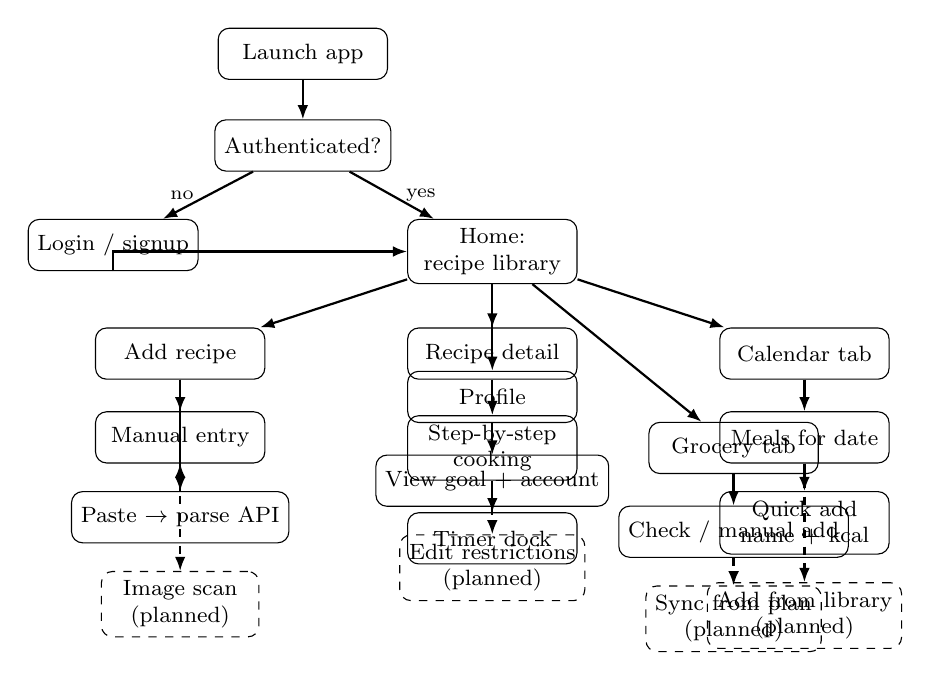
\begin{tikzpicture}[
  font=\footnotesize,
  box/.style={rectangle, draw, rounded corners, minimum width=2.15cm, minimum height=0.65cm, align=center},
  planned/.style={rectangle, draw, dashed, rounded corners, minimum width=2.0cm, minimum height=0.55cm, align=center},
  arr/.style={-{Latex[length=1.8mm]}, thick}
]
  \node[box] (launch) {Launch app};
  \node[box, below=0.5cm of launch] (auth) {Authenticated?};
  \node[box, below left=0.6cm and 0.2cm of auth] (login) {Login / signup};
  \node[box, below right=0.6cm and 0.2cm of auth] (home) {Home:\\recipe library};
  \draw[arr] (launch) -- (auth);
  \draw[arr] (auth) -- node[left, xshift=-0.05cm] {\scriptsize no} (login);
  \draw[arr] (auth) -- node[right, xshift=0.05cm] {\scriptsize yes} (home);
  \draw[arr] (login) |- (home);

  \node[box, below=0.55cm of home] (detail) {Recipe detail};
  \node[box, below=0.45cm of detail] (cook) {Step-by-step\\cooking};
  \node[box, below=0.4cm of cook] (dock) {Timer dock};
  \draw[arr] (home) -- (detail);
  \draw[arr] (detail) -- (cook);
  \draw[arr] (cook) -- (dock);

  \node[box, left=1.8cm of detail] (add) {Add recipe};
  \node[box, below=0.4cm of add] (manual) {Manual entry};
  \node[box, below=0.35cm of manual] (parse) {Paste $\rightarrow$ parse API};
  \node[planned, below=0.35cm of parse] (img) {Image scan\\(planned)};
  \draw[arr] (home) -- (add);
  \draw[arr] (add) -- (manual);
  \draw[arr] (add) -- (parse);
  \draw[arr] (parse) -- (manual);
  \draw[arr, dashed] (add) -- (img);

  \node[box, right=1.8cm of detail] (cal) {Calendar tab};
  \node[box, below=0.4cm of cal] (meals) {Meals for date};
  \node[box, below=0.35cm of meals] (quick) {Quick add\\name + kcal};
  \node[planned, below=0.35cm of quick] (lib) {Add from library\\(planned)};
  \draw[arr] (home) -- (cal);
  \draw[arr] (cal) -- (meals);
  \draw[arr] (meals) -- (quick);
  \draw[arr, dashed] (meals) -- (lib);

  \node[box, right=0.9cm of cook] (groc) {Grocery tab};
  \node[box, below=0.4cm of groc] (guse) {Check / manual add};
  \node[planned, below=0.35cm of guse] (sync) {Sync from plan\\(planned)};
  \draw[arr] (home) -- (groc);
  \draw[arr] (groc) -- (guse);
  \draw[arr, dashed] (guse) -- (sync);

  \node[box, below=1.1cm of home] (prof) {Profile};
  \node[box, below=0.4cm of prof] (pview) {View goal + account};
  \node[planned, below=0.35cm of pview] (edit) {Edit restrictions\\(planned)};
  \draw[arr] (home) -- (prof);
  \draw[arr] (prof) -- (pview);
  \draw[arr, dashed] (pview) -- (edit);
\end{tikzpicture}%
}
\caption{User flow emphasizing implemented paths; dashed nodes are planned or partial.}
\label{fig:flow}
\end{figure*}

\begin{figure}[!htb]
\centering
\resizebox{\columnwidth}{!}{%
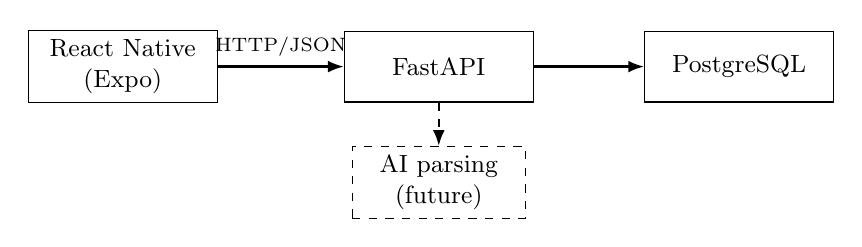
\begin{tikzpicture}[
  font=\small,
  srv/.style={rectangle, draw, minimum width=2.4cm, minimum height=0.9cm, align=center},
  future/.style={rectangle, draw, dashed, minimum width=2.2cm, minimum height=0.75cm, align=center},
  arr/.style={-{Latex[length=2mm]}, thick}
]
  \node[srv] (rn) {React Native\\(Expo)};
  \node[srv, right=1.6cm of rn] (api) {FastAPI};
  \node[srv, right=1.4cm of api] (db) {PostgreSQL};
  \node[future, below=0.55cm of api] (ai) {AI parsing\\(future)};
  \draw[arr] (rn) -- node[above, font=\scriptsize] {HTTP/JSON} (api);
  \draw[arr] (api) -- (db);
  \draw[arr, dashed] (api) -- (ai);
\end{tikzpicture}%
}
\caption{System context: mobile client, API layer, database; optional AI service for parsing.}
\label{fig:arch}
\end{figure}


\section{Project Progress Timeline}
Table~\ref{tab:gantt} summarizes major phases and status as of the progress report. Dates are illustrative for Spring~2026; adjust to your group's actual calendar. The course progress report is due March~26,~2026; final project documentation was referenced for early May in the original proposal.

\begin{table*}[!t]
\centering
\caption{Milestone summary (Spring 2026, indicative dates).}
\label{tab:gantt}
\begin{tabular}{@{}p{0.34\textwidth}p{0.12\textwidth}p{0.18\textwidth}p{0.28\textwidth}@{}}
\toprule
\textbf{Phase / task} & \textbf{Status} & \textbf{Span (approx.)} & \textbf{Notes} \\
\midrule
Proposal and wireframe & Done & Feb 1--14 & Scope and specs \\
Figma refinement & Active & Mar 1--20 & Visual and interaction exploration \\
Backend API and database & Done & Feb 15--Mar 7 & Models, migrations, routers \\
Auth and profile read & Done & Feb 20--Mar 5 & JWT, \texttt{/users/me} \\
Recipe library and detail & Done & Feb 25--Mar 10 & List, detail, navigation \\
Cooking mode and timer dock & Done & Mar 1--Mar 14 & Steps, \texttt{TimerDock} \\
Add recipe (manual + mock parse) & Done & Mar 5--Mar 15 & Verify-and-edit path \\
Meal plan API and calendar UI & Done & Mar 8--Mar 18 & Quick-add list UI \\
Grocery list basic CRUD & Done & Mar 10--Mar 18 & Sections, check, manual add \\
\midrule
Search, filter, month calendar & Active & Mar 15--Mar 29 & Close Home/Calendar gaps \\
Plan from library + grocery sync & Planned & Mar 20--Apr 7 & Aggregation design \\
Real AI text parsing & Planned & Mar 25--Apr 8 & Replace mock service \\
Profile editing and export & Planned & Apr 1--Apr 15 & PATCH user, share sheet \\
\midrule
Usability tests on build & Planned & Apr 5--Apr 15 & Scripted tasks \\
Heuristics and accessibility & Planned & Apr 12--Apr 20 & WCAG-oriented fixes~\cite{wcag21} \\
Final demo preparation & Planned & Apr 18--Apr 28 & Presentation and polish \\
Final documentation deadline & Milestone & May 3 & Final report (syllabus) \\
\bottomrule
\end{tabular}
\end{table*}

\paragraph{Risks}
Parser quality and meal--grocery integration depend on schema decisions; parallel API work with UI prototypes reduces blocking before usability tests.


\section{Conclusion}
SimpleChef has progressed from design specification to a \textbf{functional vertical prototype}: authenticated users can browse recipes, inspect detail, run step-by-step cooking with a timer dock, add recipes manually or via a parse-then-edit path, log quick meals for a date, and maintain a grocery list. The largest remaining gaps versus the proposal are search and filter on Home, a month-based planner with recipe assignment, grocery aggregation from plans, real parsing, per-step mise en place, and profile editing---together with evaluation activities (usability testing, heuristic review, accessibility) ahead of final delivery.


\bibliographystyle{IEEEtran}
\bibliography{references}

\end{document}
